\documentclass[12pt]{article}
\usepackage[top=3cm, bottom=2.5cm, left=2cm, right=2.5cm]{geometry}
\usepackage{listings}
\usepackage{float}
\usepackage{subfig}
\usepackage{graphicx}
\usepackage{ptext}
\usepackage{amsmath}
\usepackage[usenames,dvipsnames]{color,xcolor}
\usepackage{xepersian}
\setlatintextfont[Scale=1]{Times New Roman}
\settextfont[Scale=1]{XB Niloofar}


\title{تمرین سری دوم درس هوش محاسباتی}
\author{کورش تقی پور پاسدار 
\lr{400521207}}
\makeglossary
\begin{document}
	\maketitle
	\tableofcontents
	\newpage
	\section{سوال اول}
	\subsection{بخش \lr{a}}
	در شبکه‌های \lr{MLP} که توابع فعالسازی ندارند، ساختار شبکه بصورت چند لایه خطی متصل به هم می‌باشد که از نظر ریاضی اثبات می‌شود چند لایه خطی پشت سر هم، مانند یک لایه خطی عمل می‌کنند و به عبارت دیگر، یک شبکه با چند لایه خطی پشت سر هم و بدون تابع فعالسازی، مانند یک شبکه با تنها یک لایه خطی عمل می‌کند و تنها قادر به جداسازی خطی می‌باشد. درحالی که وجود توابع فعالسازی (مانند \lr{ReLU, tanh, sigmoid}) سبب غیرخطی شدن تابع شبکه شده و شبکه را پیچیده‌تر می‌کند.
	\subsection{بخش \lr{b}}
	هر تابع غیرخطی نمی‌تواند به عنوان تابع فعالسازی مورد استفاده قرار بگیرد. در انتخاب تابع فعالسازی باید به نکاتی توجه داشته باشیم:
	
	\textbf{مشتق پذیری : }درصورتی‌که تابع فعالسازی مشتق‌پذیر نباشد نمی‌توان از آن در روش‌های بهینه‌سازی مبتنی بر \lr{Back Propagation} استفاده کرد.
	
	\textbf{محدودیت دامنه : }برخی توابع مانند\lr{Sigmoid} یا \lr{tanh} خروجی را به یک بازه محدود می‌کنند که به پایداری شبکه کمک می‌کند.
	
	\textbf{پیشگیری از محو شدن گرادیان : }برخی توابع فعالسازی مانند \lr{ReLU} بدلیل ویژگی‌های خود از  مشکل محو شدن گرادیان جلوگیری کرده و به یادگیری کمک می‌کنند.
	\subsection{بخش \lr{c}}
	\subsubsection{مزایا}
	افزودن لایه‌های بیشتر سبب پیچیده‌تر شدن مدل و در نتیجه، توانایی بیشتر آن در تشخیص الگوهای پیچیده‌تر و استفاده آن در مسائل دشوارتر باشد. همچنین در ابتدا، یکی از راهکار‌های پیچیده‌تر کردن مدل، عریض‌تر کردن لایه‌ها بود. افزایش لایه‌ها بر این راهکار غلبه کرده و سبب شده تا همزمان با افزایش کمتر مقدار نورون‌ها نسبت به راهکار دیگر و کاهش هزینه‌های محاسباتی و حافظه‌ای، مدلی با قدرت بهتر ارائه دهد.
	\subsubsection{معایب}
	افزودن لایه‌های بیشتر سبب افزایش تعداد نورون‌ها و همچنین افزایش هزینه محاسباتی و حافظه‌ای مدل می‌شود. از طرفی، مدل پیچیده‌تر شده و نیاز به مجموعه داده بیشتری برای آموزش بهتر است. همچنین با پیچیده‌تر شدن مدل، احتمال \lr{overfit} مدل افزایش می‌یابد و نیاز به ارائه راهکار برای جلوگیری از آن هستیم. همچنین بدلیل وقوع \lr{Gradient Vanishing}، احتمال آموزش دیرتر و کندتر نورون‌های لایه‌های ابتدایی‌تر هستیم. همچنین تنظیم پارامترهای شبکه‌های عمیق‌تر پیچیره‌تر بوده و نیازمند آزمایش و تجربه بیشتری هستیم.
	\subsection{بخش \lr{d}}
	\subsubsection{تابع \lr{ReLU}}
	فرمول این تابع بصورت $ReLU(x) = max(0, x)$ می‌باشد و نمودار آن بصورت زیر است.
	\begin{figure}[H]
		\centering
		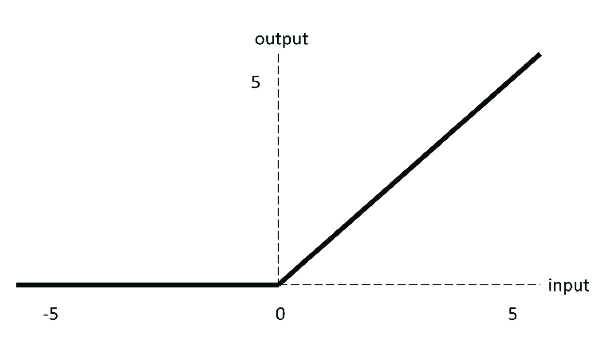
\includegraphics[scale=0.3]{pic_4.png}
	\end{figure}
	از مزایای آن می‌توان به محاسبات ساده و سریع آن اشاره کرد. همچنین به دلیل مشتق ثابت در نواحی مثبت، از ناپدید شدن گرادیان در لایه‌های عمیق‌تر پیشگیری می‌کند و سبب یادگیری بهتر مدل می‌شود. از معایب آن می‌توان به مشتق صفر در نواحی منفی اشاره کرد و همچنین اینکه خروجی آن بدون محدودیت بوده و می‌تواند مقادیر بسیار بزرگ را خروجی دهد.
	\subsubsection{تابع \lr{Sigmoid}}
	فرمول این تابع بصورت $Sigmoid(x) = \frac{1}{1+e^{-x}}$ می‌باشد و نمودار آن بصورت زیر می‌باشد.
	\begin{figure}[H]
		\centering
		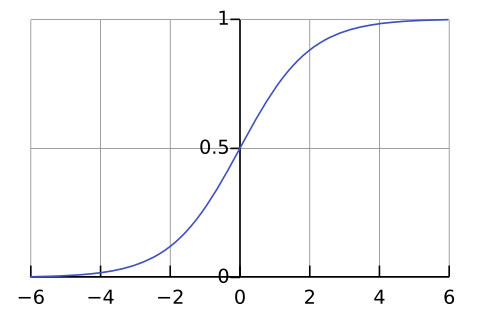
\includegraphics[scale=0.5]{pic_2.png}
	\end{figure}
	از مزایای آن می‌توان به خروجی محدود آن (در بازه ۰ و ۱) اشاره کرد و همچنین برای دسته‌بندی دوتایی (\lr{Binary Classification}) مناسب می‌باشد.از معایب آن نیز به محاسبات پیچیده‌تر آن نسبت به \lr{ReLU} , کوچک شدن گرادیان در نواحی اشباع اشاره کرد.
	\subsubsection{تابع \lr{Tanh}}
	فرمول این تابع بصورت $f(x) = \frac{e^{x} - e^{-x}}{e^{x} + e^{-x}}$ می‌باشد و نمودار آن بصورت زیر می‌باشد.
	\begin{figure}[H]
		\centering
		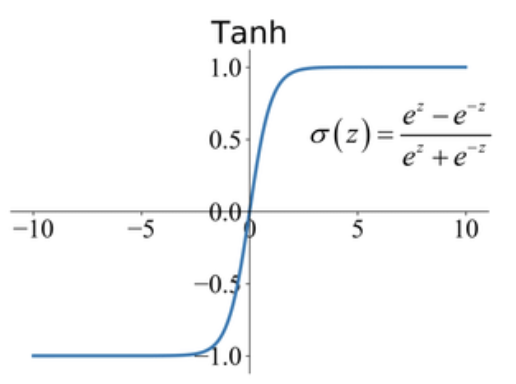
\includegraphics{pic_3.png}
	\end{figure}
	از مزایای آن می‌توان به محدود بودن خروجی‌ها اشاره کرد (بین ۱ و -۱) و همچنین خروجی ها بصورت متقارن حول صفر تعیین می‌شوند. از معایب آن نیز مشابه \lr{Sigmoid} به پیچیده‌تر بودن محاسبات نسبت به \lr{ReLU} و همچنین ناپدید شدن گرادیان در نواحی اشباع اشاره کرد.
	\subsubsection{تابع \lr{Softmax}}
	فرمول این تابع بصورت $Softmax(x) = \frac{e^{x}_{i}}{\sum_{i=1}^{n} e_{i}^{x}}$ می‌باشد. از مزایای آن می‌توان به محدود کردن خروجی به بازه ۰ تا ۱ اشاره کرد و همچنین برای دسته‌بندی چندکلاسه (\lr{Multiclass Classification}) مناسب است. از معایب آن نیز محاسبات بیشتر نسبت به سایر توابع و همچنین حساسیت نسبت به مقادیر بزرگ می‌توان گفت.
	\section{سوال دوم}
	تابع \lr{ReLU} بدلیل صفر کردن مقادیر منفی می‌تواند سبب از دست رفتن اطلاعات مهمی برای بروزرسانی شبکه شود و ممکن است که به گرادیان‌های مرده سبب شود که در آن نورون‌ها دیگر بروزرسانی نشده و فرایند آموزش متوقف می‌گردد. همچنین بدلیل استفاده همزمان از \lr{ReLU} و \lr{Sigmoid} می‌تواند شبکه را به شدت غیرخطی کرده و همگرایی را دشوار سازد. همچنین آستانه ۰.۵ می‌تواند سبب تصمیم‌گیری های نادرست شود و به عنوان مثال، هر دو خروجی ۰.۰۱ و ۰.۴۹ را به عنوان کلاس صفر خروجی دهد درحالی‌که تفاوت زیادی بین آنها وجود دارد.
	\section{سوال سوم}
	در ابتدا فرمول‌های هریک از نورون‌ها بصورت زیر نوشته می‌شود:
	
	\begin{eqnarray}
		h_{j} & = & \sum_{i=1}^n x_{i}w_{ij} \\
		y_{j} & = & \sum_{i=1}^m h_{i}w_{ij} \\
		Sigmoid & = & \frac{1}{1 + e^{-x}}
	\end{eqnarray}
	در ابتدا \lr{forward feed} حساب می‌شود.
	\begin{eqnarray}
		input 1 :&h_{1}&=Sigmoid(3 \times 6 + 1 \times -6)= 0.99\\
		 &h_{2}&=Sigmoid(3\times-3+1\times5)=0.01 \\
		 &y_{1}&=Sigmoid(h_{1}\times1+h_{2}\times0.25)=0.73\\
		 &y_{2}&=Sigmoid(h_{1}\times-2+h_{2}\times2)=0.27\\
		 input 2 :&h_{1}&=Sigmoid(-1\times6+4\times-2)=0.01\\
		 &h_{2}&=Sigmoid(-1\times-3+4\times5)=0.99\\
		 &y_{1}&=Sigmoid(h_{1}\times1+h_{2}\times0.25)=0.56\\
		 &y_{2}&=Sigmoid(h_{1}\times-2+h_{2}\times2)=0.88
	\end{eqnarray}
	حال به محاسبه \lr{Backpropagation} می‌پردازیم. در ابتدا، وزن‌ها را مطابق با شکل زیر نام‌گذاری می‌کنیم.
	\begin{figure}[H]
		\centering
		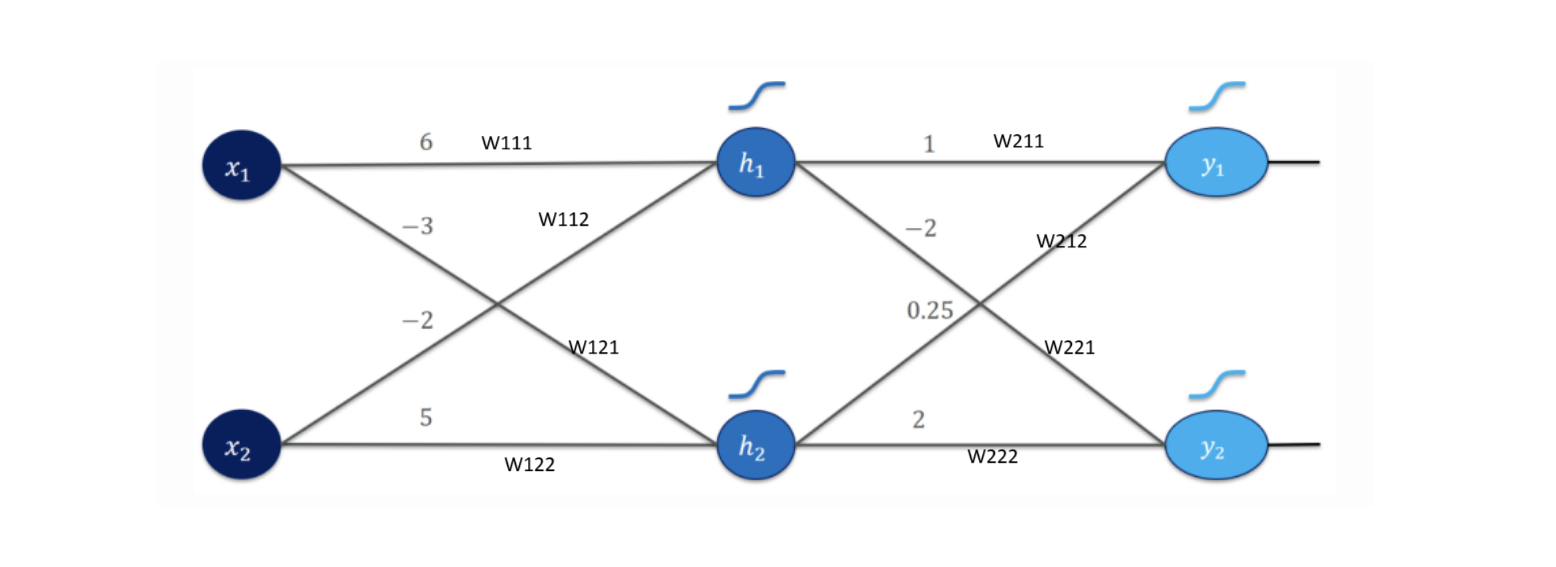
\includegraphics[scale=0.3]{pic_1.png}
	\end{figure}
	حال مراحل محاسبه آموزش وزن‌ها به صورت زیر است. همچنین نرخ آموزش بدلیل عدم ذکر در صورت سوال برابر با \lr{0.1} درنظر گرفته می‌شود.
	
	در ابتدا حالت کلی فرمول‌ها بیان می‌شود سپس به محاسبه گرادیان‌ها می‌پردازیم.
	\begin{eqnarray*}
		\Delta W_{2**} &=& lr\times Sigmoid \times (1-Sigmoid) \times (d-y) \times h\\
		\Delta W_{1**} &=& lr \times ((d_{1} - y_{1} )\times Sigmoid\times(1-Sigmoid)\times W_{2**} \\
		&+& (d_{0} - y_{0}) \times Sigmoid\times(1-Sigmoid)\times W_{2**})\times h
	\end{eqnarray*}
	\begin{eqnarray*}
	input 1 :\Delta W_{211}&=&0.1\times0.73\times0.27\times(1-0.73)\times0.99=5.26\times10^{-3}\\
	\Delta W_{212}&=&0.1\times0.73\times0.27\times(1-0.73)\times0.01=5.32\times10^{-5}\\
	\Delta W_{221}&=&0.1\times0.27\times0.73\times(0-0.27)\times0.99=-5.26\times10^{-3}\\
	\Delta W_{222}&=&0.1\times0.27\times0.73\times(0-0.27)\times0.01=-5.32\times10^{-5}\\
	%Below weights should be calculated more carefully.
	\Delta W_{111}&=&0.1\times(((1-0.73)\times0.73\times0.27\times1+(0-0.27)\times0.27\times0.73\times-2)\\
	&\times&0.99\times0.01\times3)=4.74\times10^{-4}\\	
	\Delta 
	W_{112}&=&0.1\times(((1-0.73)\times0.73\times0.27\times1+(0-0.27)\times0.27\times0.73\times-2)\\
	&\times&0.99\times0.01\times1)=1.58\times10^{-4}\\
	\Delta
	W_{121}&=&0.1\times(((1-0.73)\times0.73\times0.27\times0.25+(0-0.27)\times0.27\times0.73\times2)\\
	&\times&0.01\times0.99\times3)=-2.76\times10^{-4}\\
	\Delta
	W_{122}&=&0.1\times(((1-0.73)\times0.73\times0.27\times0.25+(0-0.27)\times0.27\times0.73\times2)\\
	&\times&0.01\times0.99\times1)=9.21\times10^{-5}\\
	input 2 :\Delta W_{211}&=&0.1\times0.56\times0.44\times(0-0.56)\times0.01=-1.37\times10^{-4}\\
	\Delta W_{212}&=&0.1\times0.56\times0.44\times(0-0.56)\times0.99=-1.36\times10^{-2}\\
	\Delta W_{221}&=&0.1\times0.88\times0.12\times(1-0.88)\times0.01=1.26\times10^{-5}\\
	\Delta W_{222}&=&0.1\times0.88\times0.12\times(1-0.88)\times0.99=1.25\times10^{-3}\\
	\Delta W_{111}&=&0.1\times(((0-0.56)\times0.56\times0.44\times1+(1-0.88)\times0.88\times0.12\times-2)\\
	&\times&0.99\times0.01\times-1)=1.61\times10^{-4}\\	
	\Delta W_{112}&=&0.1\times(((0-0.56)\times0.56\times0.44\times1+(1-0.88)\times0.88\times0.12\times-2)\\
	&\times&0.99\times0.01\times4)=-6.46\times10^{-4}\\	
	\Delta
	W_{121}&=&0.1\times(((0-0.56)\times0.56\times0.44\times0.25+(1-0.88)\times0.88\times0.12\times2)\\
	&\times&0.99\times0.01\times-1)=9.06\times10^{-6}\\
	\Delta W_{122}&=&0.1\times(((0-0.56)\times0.56\times0.44\times0.25+(1-0.88)\times0.88\times0.12\times2)\\
	&\times&0.99\times0.01\times4)=-3.62\times10^{-5}
	\end{eqnarray*}
	حال به آپدیت وزن‌ها درحالت چندتایی (\lr{Batch Mode}) می‌پردازیم. فرمول کلی آپدیت وزن‌ها بصورت $$W = W+ \sum_{x}\Delta W^{x}$$ است. وزن‌های آپدیت شده را در ادامه خواهیم داشت.
	\begin{eqnarray*}
		W_{111} &=& 6 + (4.74\times10^{-4} + 1.61\times10^{-4}) = 6.000635\\
		W_{112} &=& -2 + (1.58\times10^{-4} + -6.46\times10^{-4} ) = -2.000488\\
		W_{121} &=& -3 + (-2.76\times10^{-4} + 9.06\times10^{-6}) = -3.00026694\\
		W_{122} &=& 5 + (9.21\times10^{-5} + -3.62\times10^{-5}) = 5.0000559\\
		W_{211} &=& 1+(5.26\times10^{-3} + -1.37\times10^{-4}) = 1.005123\\
		W_{212} &=& 0.25+(5.32\times10^{-5} + -1.36\times10^{-2}) = 0.2364532\\
		W_{221} &=& -2 + (-5.26\times10^{-3} + 1.26\times10^{-5}) = -2.0052474\\
		W_{222} &=& 2 + (-5.32\times10^{-5} + 1.25\times10^{-3}) = 2.0011968
 	\end{eqnarray*}
	\section{سوال چهارم}
	در ابتدا بخش‌های تکمیل شده شرح داده می‌شوند. قابل به ذکر است که به دلیل اینکه بسیاری از این توابع تنها پیاده‌سازی فرمول‌های ریاضیاتی آن‌ها است و نکته خاصی در آنها وجود ندارد از توضیح صرف نظر شده و تنها تصاویر تکمیل شده آنها آورده می‌شود. همچنین فایل \lr{Jupyter} تکمیل شده آن در پوشه زیپ قرار دارد.
	\begin{figure}[H]
		\centering
		\subfloat[
		تابع \lr{ReLU}
		]{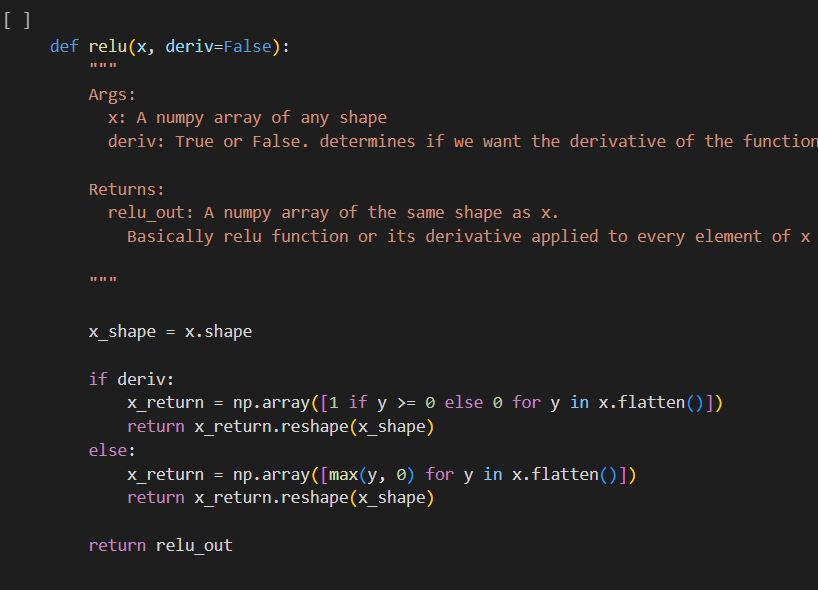
\includegraphics[height=4cm]{pic_20.png}}
		\quad \quad
		\subfloat[
		تابع \lr{Sigmoid}
		]{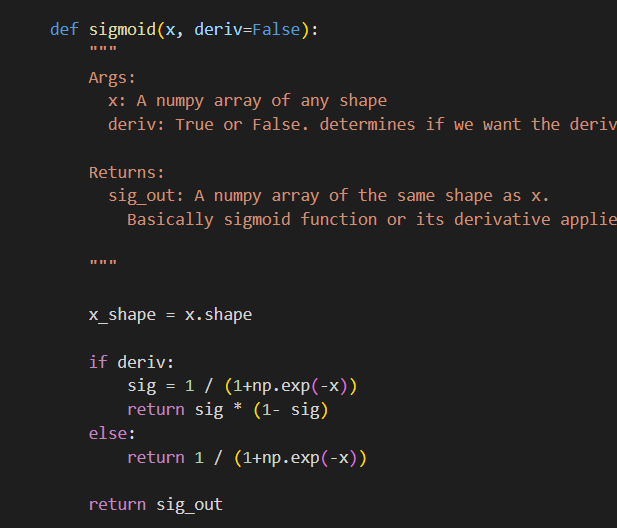
\includegraphics[height=4cm]{pic_21.png}}
		\quad \quad
		\subfloat[
		تابع \lr{feed forward}
		]{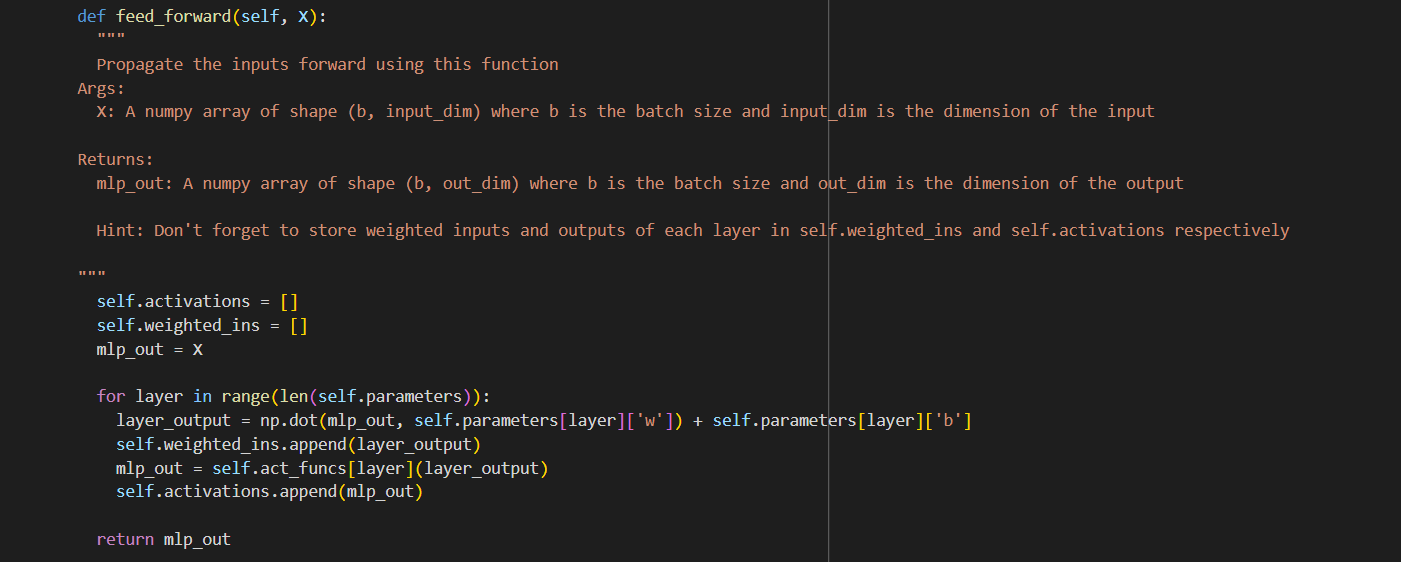
\includegraphics[height=4cm]{pic_22.png}}
		\quad \quad
		\subfloat[
		تابع \lr{Softmax}
		]{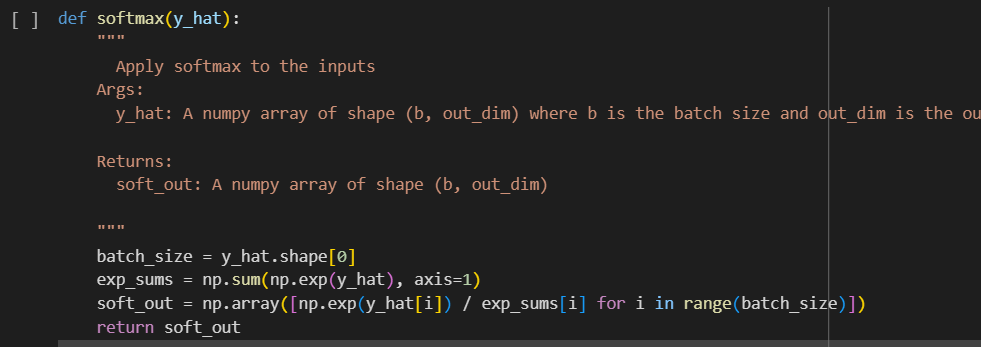
\includegraphics[height=4cm]{pic_23.png}}
		\quad \quad
		\subfloat[
		تابع \lr{Categorical Cross Entropy}
		]{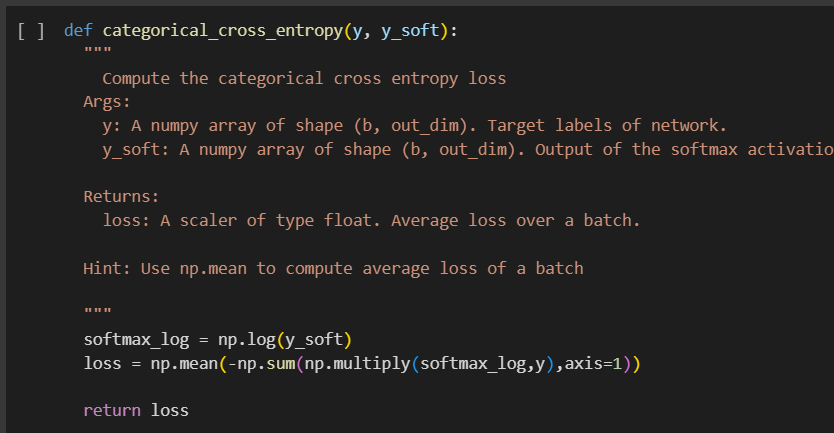
\includegraphics[height=4cm]{pic_24.png}}
		\quad \quad
		\subfloat[
		تابع \lr{Back Propagation}
		]{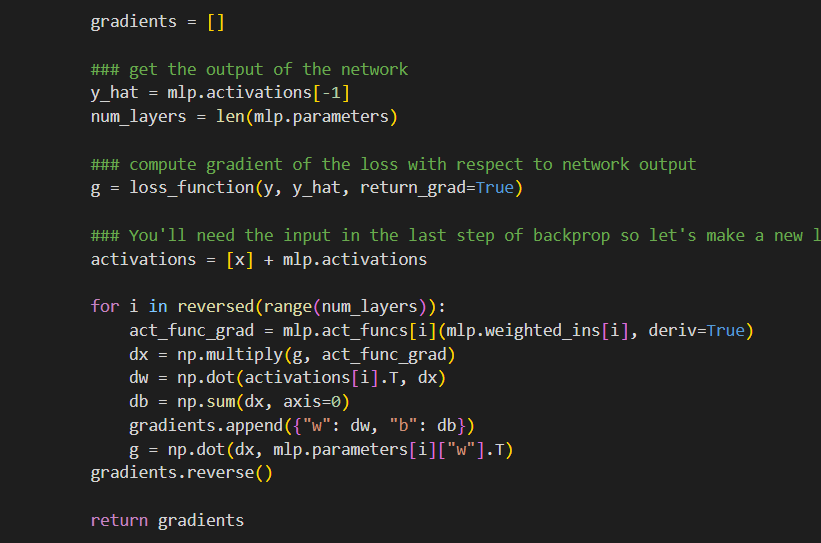
\includegraphics[height=4cm]{pic_25.png}}
		\quad \quad
		\subfloat[
		تابع \lr{Step}
		]{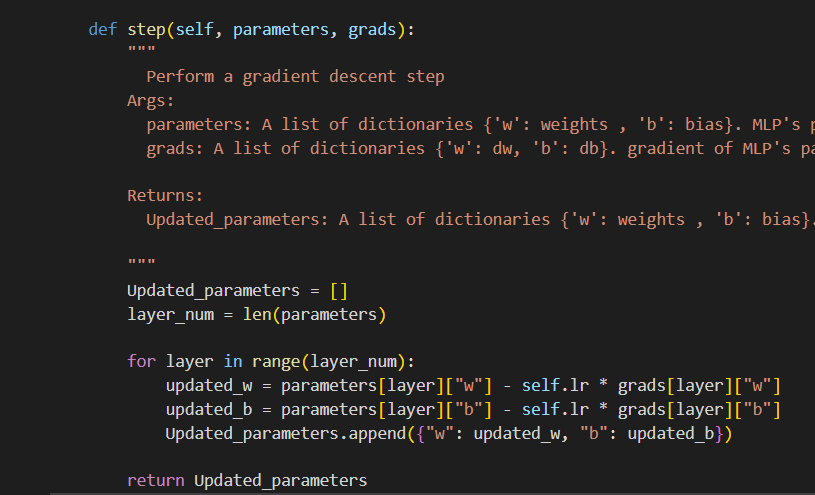
\includegraphics[height=4cm]{pic_26.png}}
		\quad \quad
		\subfloat[
		تعریف مدل \lr{MLP}
		]{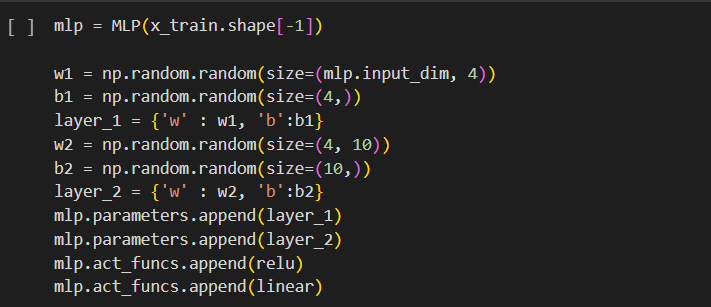
\includegraphics[height=4cm]{pic_27.png}}
	\end{figure}
	در ادامه میزان خطا، دقت و ۵ \lr{epoch} آخر را نمایش می‌دهیم. 
	\begin{figure}[H]
		\centering
		\subfloat[
		\lr{Loss}
		]{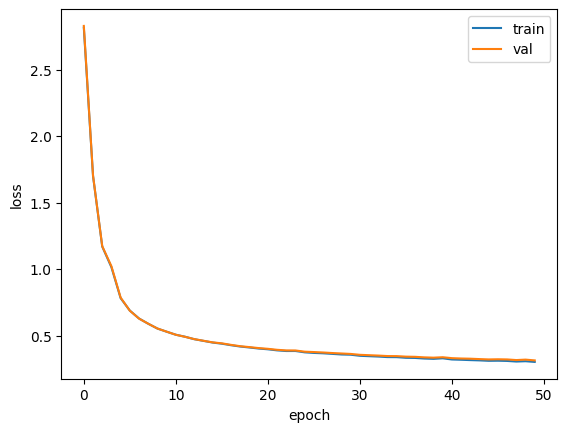
\includegraphics[height=4cm]{pic_30.png}}
		\quad \quad
		\subfloat[
		\lr{Accuracy}
		]{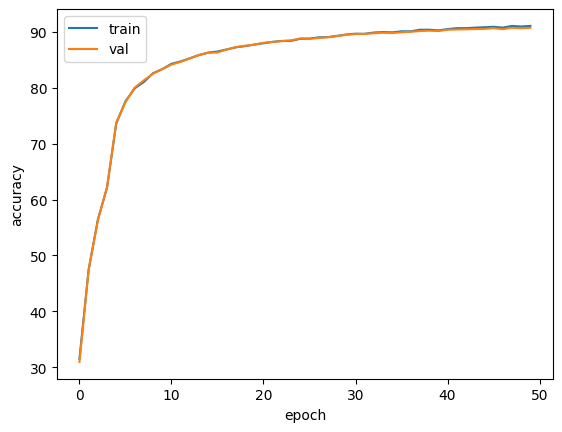
\includegraphics[height=4cm]{pic_31.png}}
		\quad \quad
		\subfloat[
		\lr{Last 5 Epochs}
		]{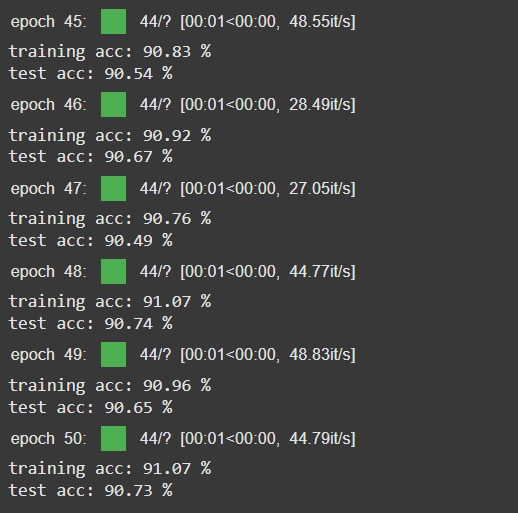
\includegraphics[height=4cm]{pic_32.png}}
	\end{figure}
	\subsection{بخش \lr{a}}
	در ابتدای کار، بجای مقداردهی رندوم وزن‌ها، آنها را با صفر مقداردهی کردیم و نمودار خطا و دقت را بدست آوردیم.
	\begin{figure}[H]
		\centering
		\subfloat[
		مقادیر خطا
		]{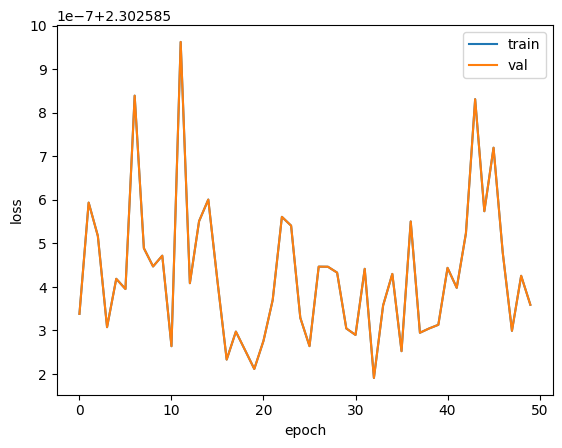
\includegraphics[height=4cm]{pic_28.png}}
		\quad \quad
		\subfloat[
		مقادیر دقت
		]{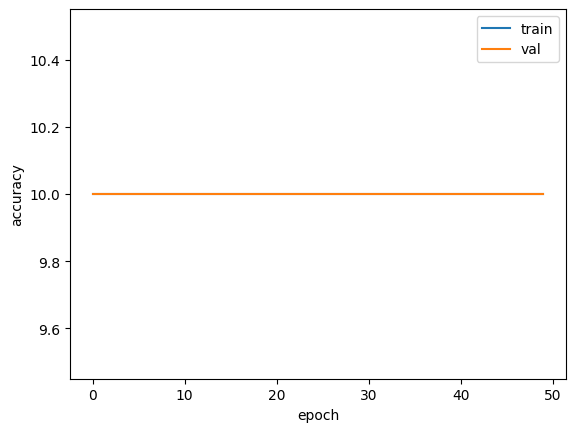
\includegraphics[height=4cm]{pic_29.png}}
	\end{figure}
	همانگونه که مشاهده می‌شود، با وزن‌دهی وزن‌ها با صفر، تمام لایه‌ها متقارن شده و خروجی لایه‌ها و مشتق به‌طورکلی صفر شده و فرآیند آموزش متوقف می‌شود.
	\subsection{بخش \lr{b}}
	در الگوریتم‌های گرادیان کاهشی، گرادیان لزوما کاهش نمی‌یابد زیرا ممکن است براثر زیاد بودن نرخ یادگیری، مدل از یک مینیمم محلی یا کلی عبور کرده یا به اصطلاح پرش کرده و به مقدار خطای بیشتری برسد که دراینصورت گرادیان بدلیل خطای بیشتر مدل در محل جدید نه تنها کاهش نیافته که افزایش نیز یافته است. این افزایش گرادیان هم می‌تواند خوب باشد (مثلا از مینیمم محلی عبور کرده و به مینیمم جهانی برسد) و هم بد باشد (در یک نقطه مناسب نتواند به مینیمم برسد و در اطراف آن پرش کند).
	\subsection{بخش \lr{c}}
	\textbf{Overfit} : در اینحالت مدل داده‌های آموزشی  را به خوبی یاد می‌گیرد ولی در داده‌های تست عملکرد ضعیفی دارد. به عبارتی مدل به جزئیات و نویزهای داده‌های آموزشی بیش از حد حساس شده است. برای رفع این مشکل می‌توان از راهکارهایی مانند کاهش پیچیدگی مدل، استفاده از \lr{Drop out} برای جلوگیری از وابستگی مدل به برخی نورون‌های خاص، استفاده از داده‌های بیشتر یا افزایش تنوع داده‌ها بهره برد.
	
	\textbf{Underfit} : در اینحالت مدل نتوانسته داده‌های آموزشی را به خوبی یاد بگیرد و در داده‌های تست نیز عملکرد ضعیفی دارد. به عبارت دیگر مدل به قدر کافی پیچیده نیست تا الگوهای موجود در داده‌ها را یاد بگیرد. برای رفع این مشکل می‌توان از پیچیده‌تر کردن مدل (افزایش تعداد لایه‌ها و نورون‌ها)، استفاده از توابع فعالسازی پیچیده‌تر، افزایش تعداد \lr{epoch} ها استفاده کرد.
	\subsection{بخش \lr{d}}
	با بررسی نمودار \lr{Loss} نهایی درمی‌یابیم که به دلیل آنکه مقدار \lr{loss} برای آموزش و تست تقریبا برابر بوده و مدل به دقت بالای ۹۰٪ دست یافته پس می‌توان گفت که مدل درحالت \lr{fit} بوده و فرآیند آموزش به خوبی پیش رفته است.
	\section{سوال پنجم}
	در ابتدا کد نوشته شده برای این سوال شرح داده می‌شود. همچنین فایل \lr{Jupyter} این سوال در پوشه زیپ شده قرار دارد.
	
	در ابتدا دیتاست \lr{Fashion MNIST} لود می‌شود و ۸ تصویر رندوم از این دیتاست نمایش داده می‌شود.
	\begin{figure}[H]
		\centering
		\subfloat[
		کد مربوط به لود کردن دیتاست و نمایش چند نمونه
		]{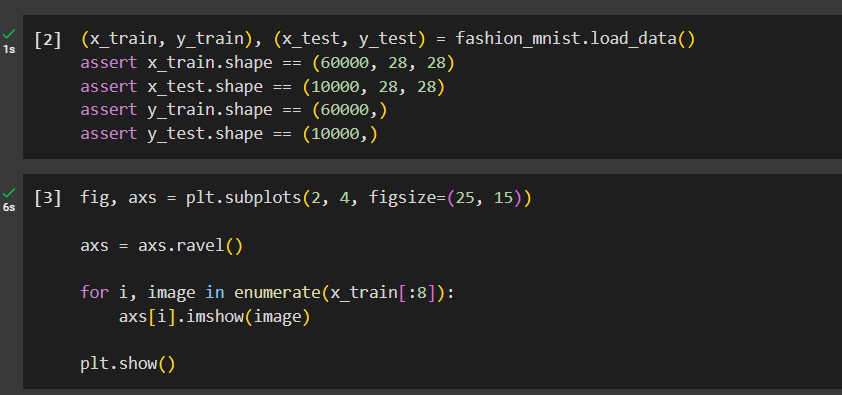
\includegraphics[scale=0.4]{pic_5.png}}
		\quad
		\subfloat[
		چند نمونه از دیتاست \lr{Fashion MNIST}
		]{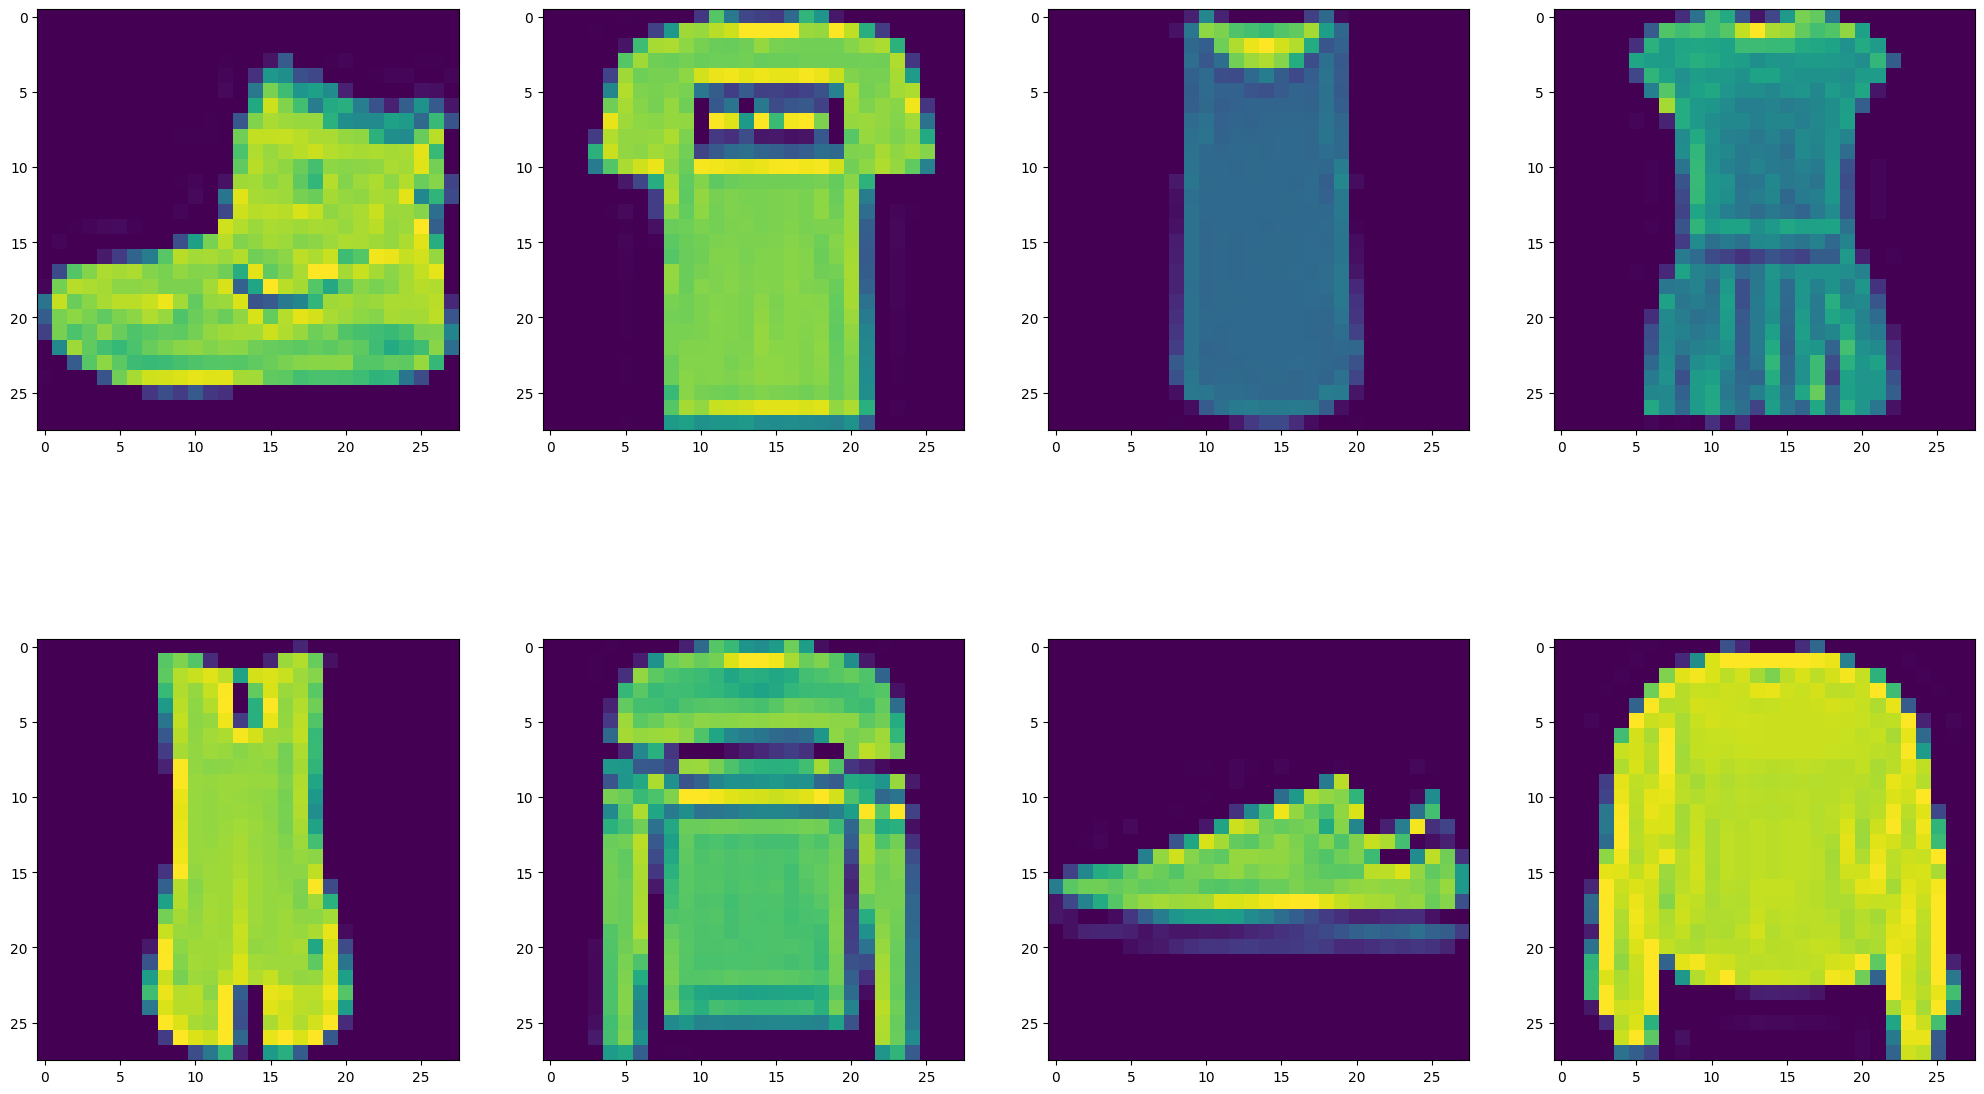
\includegraphics[scale=0.15]{pic_6.png}}
	\end{figure}
	سپس مدل را بصورت یک مدل ۵ لایه تعریف می‌کنیم که درلابه اول ۳۲ نورون، در لایه دوم و سوم ۶۴ نورون، در لایه چهارم ۳۲ نورون و درلایه پنجم و آخر ۱۰ نورون قرار دارند. همچنین توابع فعالسازی تمام لایه‌ها بجز لایه آخر \lr{ReLU} بوده و در لایه آخر تابع فعالسازی \lr{Softmax} قرار دارد (\ref{p2}). با توجه به اینکه تصاویر دیتاست از جزئیات چندان زیادی مانند رنگ، تصاویر پس زمینه و ... برخوردار نیست به‌همین دلیل تعداد نورون‌ها در لایه‌های ابتدایی چندان زیاد نیست زیرا جزئیات زیادی برای استخراج وجود ندارد. درعوض سعی شده است تا با افزایش تعداد لایه‌ها، مدل بتواند ارتباط بین این ویژگی‌ها را بهتر درک و استخراج کند. همچنین بدلیل چند کلاسه بودن مساله،‌از تابع فعالسازی \lr{Softmax} در لایه آخر استفاده شده است و برای حفظ گرادیان، در لایه‌های میانی از تابع فعالسازی \lr{ReLU} استفاده شده است. همچنین تابع ضرر مناسب برای مسائل چند کلاسه، تابع ضرر \lr{Cross Entropy} بود که استفاده شده است.
	\begin{figure}[H]
		\centering
		\subfloat[
		تعریف مدل عمیق و ترسیم پارامترهای مدل در هر لایه
		]{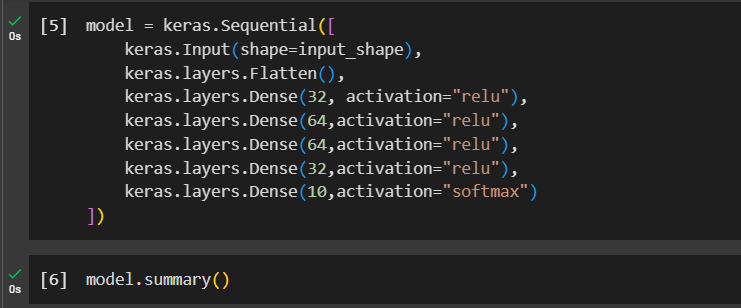
\includegraphics[scale=0.385]{pic_7.png} \label{p1}}
		\quad \quad
		\subfloat[
		ویژگی‌های مدل
		]{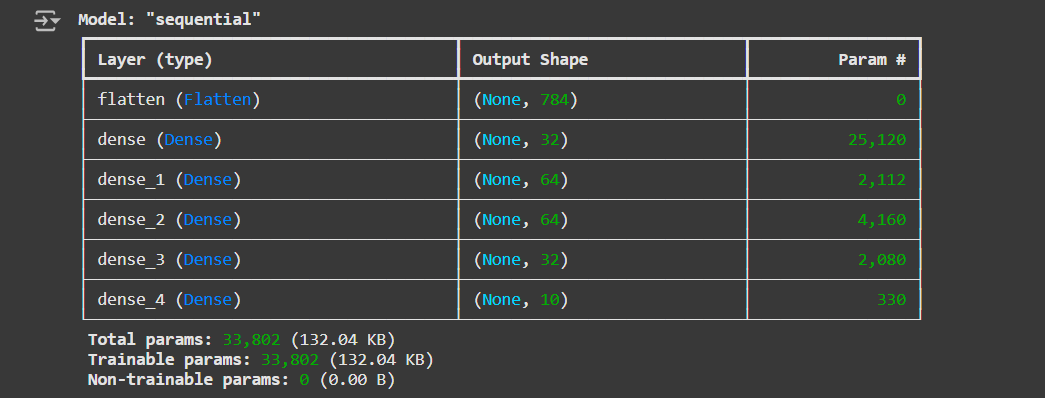
\includegraphics[scale=0.3]{pic_8.png}\label{p2}}
	\end{figure}
	سپس به آموزش مدل می‌پردازیم.
	\begin{figure}[H]
		\centering
		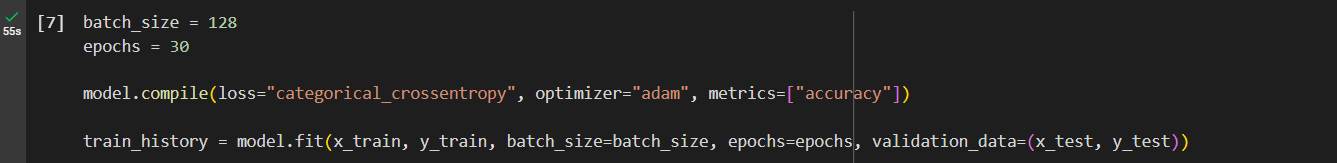
\includegraphics[scale=0.5]{pic_9.png}
	\end{figure}
	در اینجا نتیجه‌ی ۵ \lr{epoch} آخر نمایش داده شده است.
	\begin{figure}[H]
		\centering
		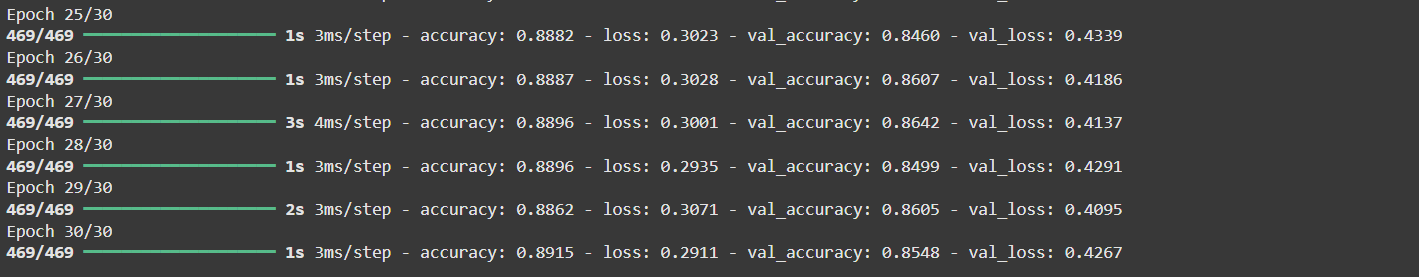
\includegraphics[scale=0.45]{pic_10.png}
	\end{figure}
	در این بخش نیز نتیجه‌ی نهایی نمایش داده می‌شود.
	\begin{figure}[H]
		\centering
		\subfloat[
		نمودار دقت مدل در هر \lr{epoch}
		]{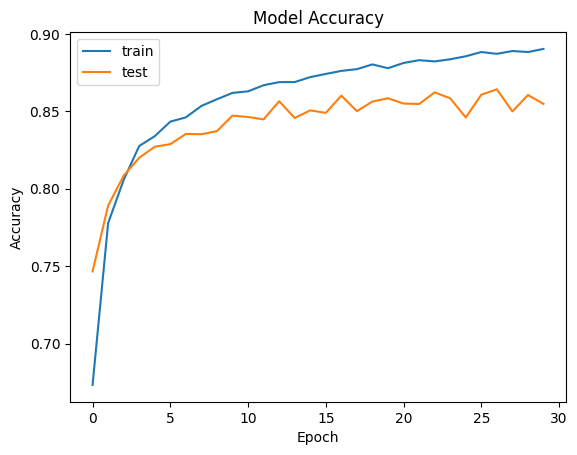
\includegraphics[scale=0.3]{pic_11.png}}
		\subfloat[
		نمودار خطای مدل در هر \lr{epoch}
		]{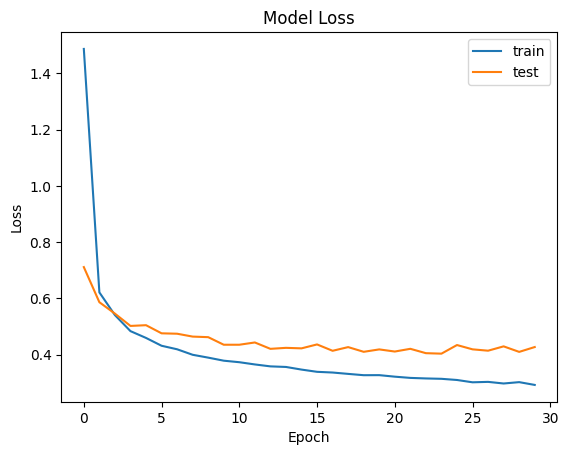
\includegraphics[scale=0.3]{pic_12.png}}
		\subfloat[
		کد مربوط به این بخش
		]{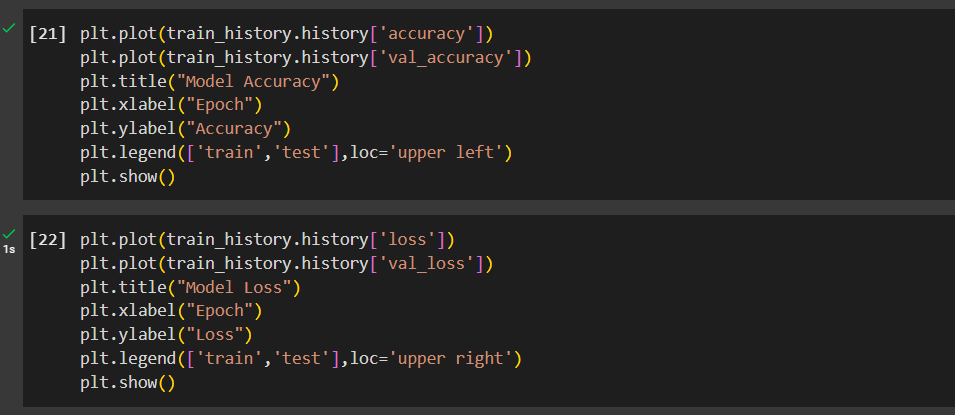
\includegraphics[scale=0.3]{pic_13.png}}
	\end{figure}
	با توجه به نمودار دقت و ضرر برای آموزش و تست، فاصله بین این دو نمودار مقدار خوب و قابل قبولی است و فاصله‌ی کم آنها نشان‌دهنده عدم رخداد \lr{overfitting} است.
	
	حال در ادامه تابع فعالسازی \lr{ReLU} با تابع فعالسازی \lr{Tanh} جایگزین می‌شود.
	\begin{figure}[H]
		\centering
		\subfloat{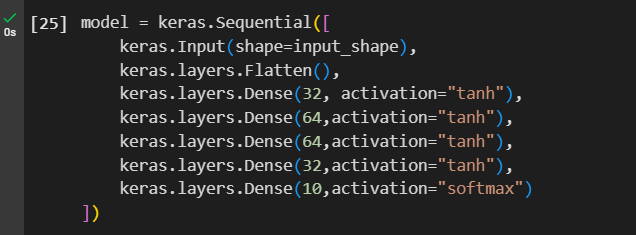
\includegraphics[scale=0.45]{pic_14.png}}
		\quad \quad 
		\subfloat{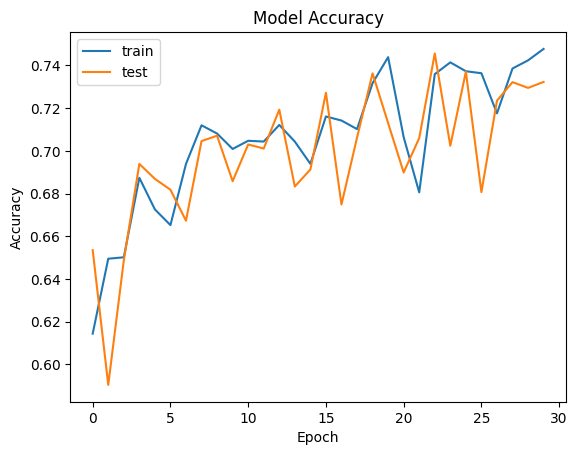
\includegraphics[scale=0.3]{pic_15.png}}
		\quad \quad 
		\subfloat{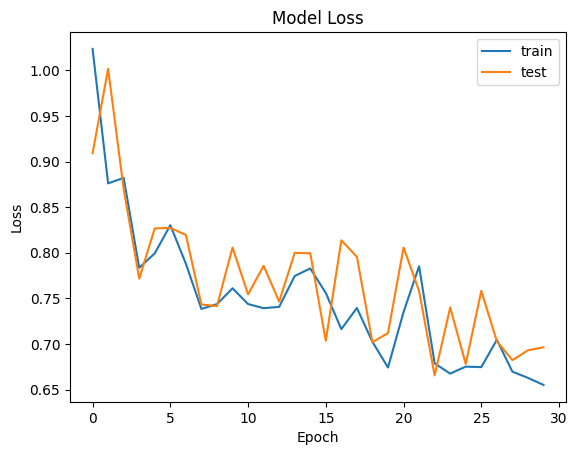
\includegraphics[scale=0.3]{pic_16.png}}
	\end{figure}
	همانطور که مشاهده می‌شود، مدل علاوه بر کاهش دقت هم در آموزش و هم تست، در این حالت رفتار‌های ناپایدارتری نیز نشان می‌دهد.
	\newline
	در ادامه بجای تابع فعالسازی \lr{ReLU} از تابع فعالسازی \lr{Sigmoid} استفاده می‌شود.
	\begin{figure}[H]
		\centering
		\subfloat{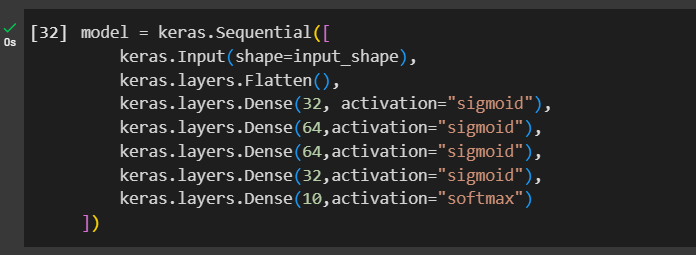
\includegraphics[scale=0.3]{pic_17.png}}
		\quad \quad
		\subfloat{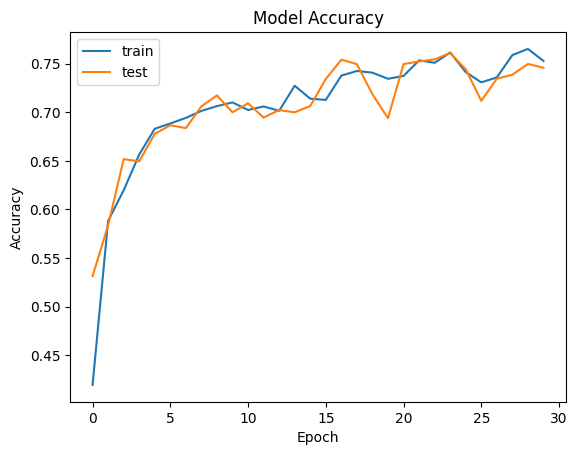
\includegraphics[scale=0.3]{pic_18.png}}
		\quad \quad
		\subfloat{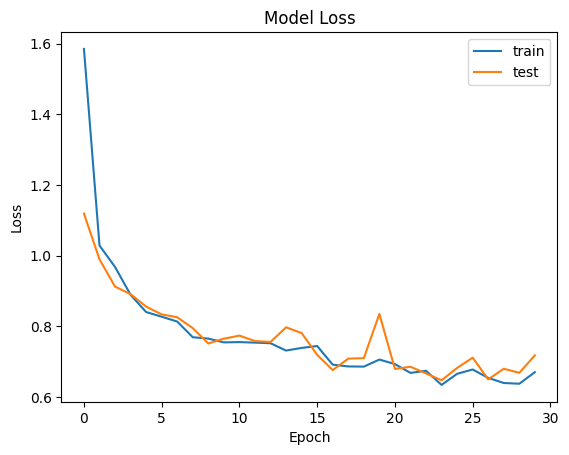
\includegraphics[scale=0.3]{pic_19.png}}
	\end{figure}
	طبق مشاهدات، مدل در این حالت بیشتر پایدار بوده ولی سرعت آموزش آن کاهش یافته است که دلیل آن مقدار کم مشتق تابع \lr{Sigmoid} می‌باشد.
\end{document}